% Meta-Informationen -------------------------------------------------------
%		Informationen über das Dokument, wie z.B. Titel, Autor, Matrikelnr. etc
%		werden in der Datei _Meta.tex definiert und können danach global
%		verwendet werden.
% --------------------------------------------------------------------------
% Informationen ------------------------------------------------------------
% 	Definition von globalen Parametern, die im gesamten Dokument verwendet
% 	werden können (z.B auf dem Deckblatt etc.).
% --------------------------------------------------------------------------
\newcommand{\titel}{End-to-End Reinforcement Learning Training of a Convolutional Neural Network to achieve an autonomous driving agent resilient to light changes}
\newcommand{\art}{Master's Thesis}
\newcommand{\ort}{Leipzig}
\newcommand{\hochschule}{Universität Leipzig}
\newcommand{\fachgebiet}{Database Department}
\newcommand{\fakultaet}{Faculty of Mathematics and Computer Science}
\newcommand{\institut}{Institute of Computer Science}
\newcommand{\autor}{Georg Schneeberger}
\newcommand{\matrikelnr}{3707914}
\newcommand{\erstbetreuer}{Prof. Dr. Erhard Rahm}
\newcommand{\zweitbetreuer}{Dr. Thomas Burghardt}
\newcommand{\drittbetreuer}{Martin Lorenz}
\newcommand{\jahr}{2024}
\newcommand{\invnr}{1337}
\newcommand{\eingereicht}{28.06.2024}

% Eigene Befehle
\newcommand{\todo}[1]{\textbf{\textsc{\textcolor{red}{(TODO: #1)}}}}

% Autorennamen in small caps
\newcommand{\AutorZ}[1]{\textsc{#1}}
\newcommand{\Autor}[1]{\AutorZ{\citeauthor{#1}}}

% Befehle zur semantischen Auszeichnung von Text
\newcommand{\NeuerBegriff}[1]{\textbf{#1}}
\newcommand{\Fachbegriff}[1]{\textit{#1}}
\newcommand{\Prozess}[1]{\textit{#1}}
\newcommand{\Webservice}[1]{\textit{#1}}
\newcommand{\Eingabe}[1]{\texttt{#1}}
\newcommand{\Code}[1]{\texttt{#1}}
\newcommand{\Datei}[1]{\texttt{#1}}
\newcommand{\Datentyp}[1]{\textsf{#1}}
\newcommand{\XMLElement}[1]{\textsf{#1}}

% Abkürzungen
\newcommand{\vgl}{Vgl.\ }
\newcommand{\ua}{\mbox{u.\,a.\ }}
\newcommand{\zB}{\mbox{z.\,B.\ }}
\newcommand{\bs}{$\backslash$}

% Einfache Anführungszeichen in texttt
\newcommand{\sq}{\textquotesingle}



% Dokumentenkopf -----------------------------------------------------------
% 	Diese Vorlage basiert auf "scrreprt" aus dem koma-script.
%		Die Option draft sollte beim fertigen Dokument ausgeschaltet werden.
% --------------------------------------------------------------------------
\documentclass[
	11pt,					% Schriftgröße
	DIV=10,
	ngerman,				% für Umlaute, Silbentrennung etc.
	a4paper,				% Papierformat
	oneside,				% einseitiges Dokument
	titlepage,				% es wird eine Titelseite verwendet
	parskip=half,			% Abstand zwischen Absätzen (halbe Zeile)
	headings=normal, % Größe der Überschriften verkleinern
	numbers=withendperiod, % Fügt in den Überschriften nach den Zahlen einen Punkt ein
	listof=totoc,				% Verzeichnisse im Inhaltsverzeichnis aufführen
	bibliography=totoc,				% Literaturverzeichnis im Inhaltsverzeichnis aufführen
	index=totoc,				% Index im Inhaltsverzeichnis aufführen
	captions=tableheading,		% Beschriftung von Tabellen oberhalb ausgeben
	final					% Status des Dokuments (final/draft)
]{scrreprt}

\renewcommand*\chapterheadstartvskip{\vspace*{-1.0cm}}

% Bentigte Packages -------------------------------------------------------
%		Weitere Packages, die benötigt werden, sind in die Datei Packages.tex
%		"ausgelagert", um die Vorlage möglichst übersichtlich zu halten.
% --------------------------------------------------------------------------
% Anpassung des Seitenlayouts ----------------------------------------------
% 	siehe Seitenstil.tex
% --------------------------------------------------------------------------
\usepackage[
	automark,			% Kapitelangaben in Kopfzeile automatisch erstellen
	headsepline,	% Trennlinie unter Kopfzeile
	ilines				% Trennlinie linksbündig ausrichten
]{scrlayer-scrpage}
\usepackage{scrhack} % Disable some warnings

\usepackage{pseudocode}
\usepackage{nicefrac}

% Für eine schöne Anordnung von Bildern
\usepackage{subfigure}

\usepackage{dsfont}
%\usepackage{color}
%
%% Define user colors using the RGB model
%\definecolor{yellow}{rgb}{0.0,1.0,0.0}
%\definecolor{rot}{rgb}{1.0,0.0,0.0}

% Anpassung an Landessprache -----------------------------------------------
% 	Verwendet globale Option german siehe \documentclass
% --------------------------------------------------------------------------
\usepackage[ngerman]{babel}

% Umlaute ------------------------------------------------------------------
% 		Umlaute/Sonderzeichen wie äöüß direkt im Quelltext verwenden (CodePage).
%		Erlaubt automatische Trennung von Worten mit Umlauten.
% --------------------------------------------------------------------------
\usepackage[utf8]{inputenc}
\usepackage[T1]{fontenc}
%\usepackage{ae} % "schöneres" ä
\usepackage{textcomp} % Euro-Zeichen etc.
\usepackage{lmodern} % schööön

% Grafiken -----------------------------------------------------------------
% 		Einbinden von Grafiken [draft oder final]
% 		Option [draft] bindet Bilder nicht ein - auch globale Option
% --------------------------------------------------------------------------
\usepackage[dvips,final]{graphicx}
\usepackage{wrapfig}
\graphicspath{{Bilder/}} % Dort liegen die Bilder des Dokuments

% Befehle aus AMSTeX für mathematische Symbole z.B. \boldsymbol \mathbb ----
\usepackage{amsmath,amsfonts,amsthm}

% Für Index-Ausgabe; \printindex -------------------------------------------
\usepackage{makeidx}

% Einfache Definition der Zeilenabstände und Seitenränder etc. -------------
\usepackage{setspace}
\usepackage{geometry}

% für gedrehte Tabellen
\usepackage{rotating} 

% Symbolverzeichnis --------------------------------------------------------
% 	Symbolverzeichnisse bequem erstellen, beruht auf MakeIndex.
% 		makeindex.exe %Name%.nlo -s nomencl.ist -o %Name%.nls
% 	erzeugt dann das Verzeichnis. Dieser Befehl kann z.B. im TeXnicCenter
%		als Postprozessor eingetragen werden, damit er nicht ständig manuell
%		ausgeführt werden muss.
%		Die Definitionen sind ausgegliedert in die Datei Abkuerzungen.tex.
% --------------------------------------------------------------------------
\usepackage[intoc]{nomencl}
  \let\abbrev\nomenclature
  \renewcommand{\nomname}{Abkürzungsverzeichnis}
  \setlength{\nomlabelwidth}{.25\hsize}
  \renewcommand{\nomlabel}[1]{#1 \dotfill}
  \setlength{\nomitemsep}{-\parsep}

% Zum Umfließen von Bildern -------------------------------------------------
\usepackage{floatflt}

% Zum Einbinden von Programmcode --------------------------------------------
\usepackage{listings}
\usepackage{xcolor} 
\definecolor{hellgelb}{rgb}{1,1,0.9}
\definecolor{colKeys}{rgb}{0,0,1}
\definecolor{colIdentifier}{rgb}{0,0,0}
\definecolor{colComments}{rgb}{1,0,0}
\definecolor{colString}{rgb}{0,0.5,0}
\lstset{%
    float=hbp,%
    basicstyle=\texttt\small, %
    identifierstyle=\color{colIdentifier}, %
    keywordstyle=\color{colKeys}, %
    stringstyle=\color{colString}, %
    commentstyle=\color{colComments}, %
    columns=flexible, %
    tabsize=2, %
    frame=single, %
    extendedchars=true, %
    showspaces=false, %
    showstringspaces=false, %
    numbers=left, %
    numberstyle=\tiny, %
    breaklines=true, %
    backgroundcolor=\color{hellgelb}, %
    breakautoindent=true, %
%    captionpos=b%
}

% Lange URLs umbrechen etc. -------------------------------------------------
\usepackage{url}


\usepackage{makecell}

%% Wichtig für korrekte Zitierweise ------------------------------------------

\usepackage[autocite=inline, sorting=none]{biblatex}
\bibliography{quellen} % Name der .bib-Datei

\usepackage{csquotes} % Empfohlen, um Zitierten Text richtig darzustellen

% ermöglicht Zeilenumbrüche in Captions
\usepackage{caption}


% PDF-Optionen --------------------------------------------------------------
\usepackage[
bookmarks,
bookmarksopen=true,
pdftitle={\titel},
pdfauthor={\autor},
pdfcreator={\autor},
pdfsubject={\titel},
pdfkeywords={\titel},
colorlinks=true,
%linkcolor=red, % einfache interne Verknüpfungen
%anchorcolor=black,% Ankertext
%citecolor=blue, % Verweise auf Literaturverzeichniseinträge im Text
%filecolor=magenta, % Verknüpfungen, die lokale Dateien öffnen
%menucolor=red, % Acrobat-Menüpunkte
%urlcolor=cyan, 
% für die Druckversion können die Farben ausgeschaltet werden:
linkcolor=black, % einfache interne Verknüpfungen
anchorcolor=black,% Ankertext
citecolor=black, % Verweise auf Literaturverzeichniseinträge im Text5
filecolor=black, % Verknüpfungen, die lokale Dateien öffnen
menucolor=black, % Acrobat-Menüpunkte
urlcolor=black, 
%backref,
%pagebackref,
plainpages=false,% zur korrekten Erstellung der Bookmarks
pdfpagelabels,% zur korrekten Erstellung der Bookmarks
hypertexnames=false,% zur korrekten Erstellung der Bookmarks
linktocpage % Seitenzahlen anstatt Text im Inhaltsverzeichnis verlinken
]{hyperref}

% Zum fortlaufenden Durchnummerieren der Fußnoten ---------------------------
\usepackage{chngcntr}


% für lange Tabellen
\usepackage{longtable}
\usepackage{array}
\usepackage{ragged2e}
\usepackage{lscape}

\usepackage{supertabular}

% Spaltendefinition rechtsbündig mit definierter Breite ---------------------
\newcolumntype{w}[1]{>{\raggedleft\hspace{0pt}}p{#1}}

% Formatierung von Listen ändern
\usepackage{paralist}
% Standardeinstellungen:
% \setdefaultleftmargin{2.5em}{2.2em}{1.87em}{1.7em}{1em}{1em}

\usepackage{tablefootnote}
% für Ausblenden der Seitenzahl
\usepackage{lipsum}

% Erstellung eines Index und Abkürzungsverzeichnisses aktivieren -----------
\makeindex
% makeindex Masterarbeit.nlo -s nomencl.ist -o Masterarbeit.nls
\makenomenclature


% Kopf- und Fußzeilen, Seitenränder etc. -----------------------------------
% Zeilenabstand ------------------------------------------------------------
\onehalfspacing 
% \setstretch{1,5}

% Seitenränder -------------------------------------------------------------
\geometry{paper=a4paper,left=25mm,right=20mm,top=20mm, bottom=25mm}
% Notfall maße :)
%\geometry{paper=a4paper,left=35mm,right=25mm,top=25mm, bottom=25mm}



% Kopf- und Fußzeilen ------------------------------------------------------
\pagestyle{scrheadings}

% Kopf- und Fußzeile auch auf Kapitelanfangsseiten -------------------------
\renewcommand*{\chapterpagestyle}{scrheadings}

% Schriftform der Kopfzeile ------------------------------------------------
\renewcommand{\headfont}{\normalfont}

% Kopfzeile ----------------------------------------------------------------
\ihead{\textit{\headmark}}
\chead{}
%\ohead{\includegraphics[scale=1]{Bilder/logoKlein.JPG}}
\ohead{}
\setlength{\headheight}{8mm} % Höhe der Kopfzeile
\setheadwidth[0pt]{textwithmarginpar} % Kopfzeile über den Text hinaus verbreitern

% Fußzeile -----------------------------------------------------------------
% \ifoot{\copyright\ \autor \\ \invnr}
% \ifoot{\copyright\ \autor \\ \matrikelnr}
\ifoot{\autor \\ \matrikelnr}
\cfoot{}
\ofoot{\pagemark}
\setlength{\footskip}{12mm}
\setfootwidth[0pt]{text}

% Überschriften ------------------------------------------------------------
\renewcommand*\chapterheadstartvskip{\vspace*{-0.5cm}} % Platz vor einer Überschrift eines neuen Kapitels


% erzeugt ein wenig mehr Platz hinter einem Punkt --------------------------
\frenchspacing

% Schusterjungen und Hurenkinder vermeiden
\clubpenalty = 10000
\widowpenalty = 10000 
\displaywidowpenalty = 10000


% Quellcode-Ausgabe formatieren --------------------------------------------
%\lstset{numbers=left, numberstyle=\tiny, numbersep=5pt, breaklines=true}
%\lstset{emph={square}, emphstyle=\color{red}, emph={[2]root,base}, emphstyle={[2]\color{blue}}}

\definecolor{gray}{rgb}{0.9,0.9,0.9}

\lstset{%
		basicstyle=\small\ttfamily,language={[LaTeX]TeX},
		numbersep=5mm, 
		numbers=left,
		numberstyle=\tiny,
		breaklines=true,
		framexleftmargin=8mm, 
		xleftmargin=8mm,
		backgroundcolor=\color{gray},
		captionpos=b
}%

% Fußnoten fortlaufend durchnummerieren ------------------------------------
\counterwithout{footnote}{chapter}

% Definitionen

\newtheorem{definition}{Definition}


% Eigene Definitionen für Silbentrennung
\hyphenation{Trenn-bar-es}

% Das eigentliche Dokument -------------------------------------------------
%		Der eigentliche Inhalt des Dokuments beginnt hier. Die einzelnen Seiten
%		und Kapitel werden in eigene Dateien ausgelagert und hier nur inkludiert.
% --------------------------------------------------------------------------

\begin{document}
% auch subsubsection nummerieren
\setcounter{secnumdepth}{3}
\setcounter{tocdepth}{3}

% keine Kopf-/Fußzeilen bei Deckblatt und Abstract
\ofoot{}
% Deckblatt
%\thispagestyle{plain}
\begin{titlepage}

\begin{center}

\includegraphics[height=7cm]{Bilder/Uni-L.png}\\[2.5ex]

\institut\\
\fakultaet\\
\fachgebiet\\[6ex]

\textbf{\large\titel}\\[1.5ex]
\art\\[6ex]

\normalsize
submitted by:\\
\autor\\[1.5ex]
matriculation number:\\
\matrikelnr\\[1.5ex]
Supervisor:\\
\erstbetreuer\\
\zweitbetreuer\\[1.0ex]
\end{center}

%\begin{tabbing}
%\hspace{3.5cm}\= \kill
%   vorgelegt von: \> \autor\\[1.2ex]
%   Matrikelnummer: \> \matrikelnr\\[1.2ex]
%    \> \\
%   Betreuer: \> \erstbetreuer\\[1.2ex]
%    \> \zweitbetreuer
%\end{tabbing}

\begin{center}
\copyright\ \jahr\\[1.0ex]
\end{center}

\singlespacing
\small
\noindent This thesis and its parts are \textbf{protected by copyright}. Any use outside the narrow limits of copyright law without the consent of the author is prohibited and punishable by law. This applies in particular to reproductions, translations, microfilming as well as storage and processing in electronic systems.

\end{titlepage}


%\section*{Abstract}
\label{sec:Abstract}

In my master's thesis I will investigate using neural networks for self driving. The goal is to create an autonomous driving agent that is resilient to changes in light conditions. The agent will employ preprocessing steps and a convolutional neural network to achieve this. The agent will be trained using reinforcement learning in a simulated environment with changing light conditions to help the agent generalize.

The reinforcement learning agent's task is to complete a parcour in a simulated environment without collisions. The thesis builds upon previous student's work at the ScaDS.AI \autocite{maximilian}, the task specifications and evaluation approaches are reused for comparability. This thesis focusses on improving the resiliency to changing light conditions.

% TODO ScaDS.AI ist die Schreibweise, wird sie auch im Text so verwendet?

% \section*{Danksagung}
\label{sec:Danksagung}
Danksagung
\newpage
\ofoot{\pagemark}

% Seitennummerierung -------------------------------------------------------
%		Vor dem Hauptteil werden die Seiten in großen römischen Ziffern 
%		nummeriert...
% --------------------------------------------------------------------------
\pagenumbering{Roman}

%\tableofcontents			% Inhaltsverzeichnis

% Abkürzungsverzeichnis ----------------------------------------------------
%\input{Inhalt/Glossar}
%\printnomenclature
%\label{sec:Glossar}

%\renewcommand{\lstlistlistingname}{Verzeichnis der Listings}
%\lstlistoflistings	

% ...danach in normalen arabischen Ziffern ---------------------------------
\clearpage
\pagenumbering{arabic}


% Inhalt -------------------------------------------------------------------
%		Hier können jetzt die einzelnen Kapitel inkludiert werden. Sie müssen
%		in den entsprechenden .TEX-Dateien vorliegen. Die Dateinamen können
% 		natürlich angepasst werden.
% --------------------------------------------------------------------------
\chapter{Methods}
\label{cha:Methods}


% Doku für APseudocode package
% https://ftp.agdsn.de/pub/mirrors/latex/dante/macros/latex/contrib/pseudocode/pseudocode.pdf

\renewcommand{\thepseudonum}{\roman{pseudonum}}
\begin{pseudocode}{Collect Data}{ }
\COMMENT{Fill RolloutBuffer with samples obtained by current model}\\

\PROCEDURE{CollectData}{}
num\_steps \GETS 0\\
RolloutBuffer.\CALL{Reset}{}\\
Env.\CALL{Reset}{}\\
\WHILE RolloutBuffer\CALL{NotFull}{} \DO
\BEGIN
obs \GETS Env.\CALL{GetObservation}{}\\
action \GETS Model.\CALL{GetAction}{obs}\\
reward \GETS Env.\CALL{Step}{action}\\
num\_steps \GETS num\_steps + 1\\
\CALL{AddToRolloutBuffer}{obs, action, reward}\\
\IF Env.\CALL{IsFinished}{} \THEN
Env.\CALL{Reset}{}\\
\END\\
\RETURN{num\_steps}
\ENDPROCEDURE

\end{pseudocode}

\begin{figure}
     \centering
     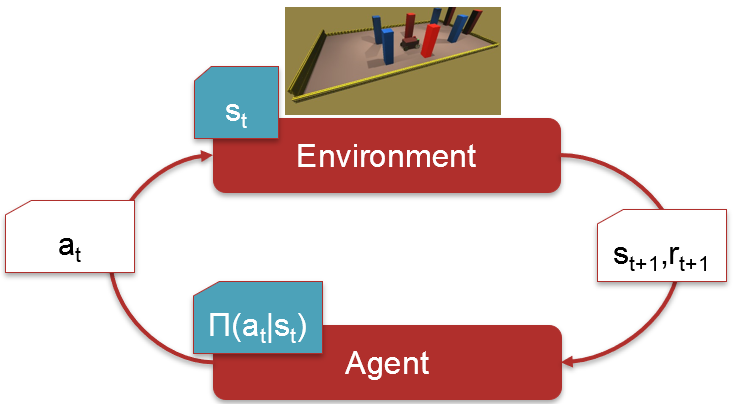
\includegraphics[width=0.8\textwidth]{Bilder/rl_cycle.png}
     \caption{Loop in Collect Data}
     \label{fig:unitycommunication}
\end{figure}


\renewcommand{\thepseudonum}{\roman{pseudonum}}
\begin{pseudocode}{Train Model}{ }
\COMMENT{Sample from replay buffer and update the model based on the loss}\\

\PROCEDURE{TrainModel}{}
amount\_of\_batches \GETS \frac{rollout\_buffer\_size}{batch\_size}\\
\FOR i \GETS 0 \TO n\_epochs \DO
\BEGIN
RolloutBuffer.\CALL{Shuffle}{}\\
\FOR i \GETS m \TO amount\_of\_batches \DO
\BEGIN
batch \GETS RolloutBuffer.\CALL{GetBatch}{m}\\
loss \GETS \CALL{ComputeLoss}{batch}\\
Model.\CALL{Backpropagate}{loss}\\
Optimizer.\CALL{Step}{}\\
\END\\
\END
\ENDPROCEDURE

\end{pseudocode}



\renewcommand{\thepseudonum}{\roman{pseudonum}}
\begin{pseudocode}{Evaluate Model}{ }
\COMMENT{Evaluate Model on tracks of all difficulties}\\

\PROCEDURE{Episode}{}
\WHILE Env.\CALL{IsFinished}{}==False \DO
\BEGIN
obs \GETS Env.\CALL{GetObservation}{}\\
action \GETS Model.\CALL{GetAction}{obs}\\
\END\\
\IF Env.\CALL{FinishedSuccessfully}{} \THEN
success \GETS 1
\ELSE
success \GETS 0\\
\RETURN{success}
\ENDPROCEDURE

\PROCEDURE{EvalModelTrack}{n\_episodes, difficulty}
successful\_episodes \GETS 0\\
\FOR episodes \GETS 0 \TO n\_episodes \DO
\BEGIN
Env.\CALL{Reset}{difficulty}\\
successful\_episodes \GETS successful\_episodes + \CALL{Episode}{}\\
\END\\
success\_rate \GETS \frac{successful\_episodes}{n\_eval\_episodes}\\
\RETURN{success\_rate}
\ENDPROCEDURE

\PROCEDURE{EvalModel}{}
easy\_success\_rate = \CALL{EvalModelTrack}{n\_episodes=num\_evals\_per\_difficulty, \\difficulty=''easy''}\\
medium\_success\_rate = \CALL{EvalModelTrack}{n\_episodes=num\_evals\_per\_difficulty, \\difficulty=''medium''}\\
hard\_success\_rate = \CALL{EvalModelTrack}{n\_episodes=num\_evals\_per\_difficulty, \\difficulty=''hard''}\\
\\
total\_success\_rate = (easy\_success\_rate + medium\_success\_rate + hard\_success\_rate) / 3\\
\IF total\_success\_rate > best\_success\_rate \THEN
\BEGIN
best\_success\_rate \GETS total\_success\_rate\\
Model.\CALL{SaveToFile}{}\\
\END
\ENDPROCEDURE
\end{pseudocode}

\renewcommand{\thepseudonum}{\roman{pseudonum}}
\begin{pseudocode}{TrainNetwork}{ }
\label{Train}
\COMMENT{Main Training Algorithm}\\

\MAIN
Env \GETS \CALL{Environment}{environment\_parameters}\\
RolloutBuffer \GETS \CALL{RolloutBuffer}{rollout\_buffer\_size}\\
Model \GETS \CALL{Model}{model\_parameters}\\
Optimizer \GETS \CALL{Optimizer}{optimizer\_parameters}\\


num\_timesteps \GETS 0\\
iteration \GETS 0\\
\WHILE num\_timesteps < total\_timesteps \DO 
\BEGIN 
num\_steps \GETS \CALL{CollectData}{}\\
num\_timesteps \GETS num\_timesteps + num\_steps\\
iteration \GETS iteration + 1\\
\CALL{TrainModel}{}\\
\IF iteration \mathbin{\%}  log\_interval = 0 \THEN
\BEGIN
success\_rate \GETS \CALL{EvalModel}{}\\
\CALL{LogToTensorboard}{key=''eval/success\_rate'', value=success\_rate,\\ step=num\_timesteps}\\
\END
\END\\
\ENDMAIN
\end{pseudocode}





\chapter{Isolierte Ergebnisse}
\label{cha:Isolierte Ergebnisse}


\subsection{reward funktionen}

Previous sections introduced the composite reward function. The composite reward function consists of a weighted sum of individual reward functions. The individual reward functions are designed to encourage the agent to learn the desired behaviour. The goal is to achieve an agent that completes the parcour without collisions, this is encapsulated in the event reward function. However the event reward function is a very spare signal, which makes it hard for the agent to learn. The other individual reward functions are designed to not be sparse, however some of these functions are not enough to guide the agent to the desired behaviour alone, such as the orientation reward.
It is important to find appropriate weights of the individual reward functions for the composite reward function. We are conducting experiments to analyse the usefullness of the individual reward functions. We analyse if the agent is capable of learning the behaviour encouraged by the reward function.

see \ref{table:reward_functions_behaviour}


\begin{table}
    
\caption{Training runs with different reward functions alone (all coefficients 0 except the one of the reward function)}
\begin{center}
\begin{tabular}{|| c | c | c | c ||} 
    \hline
    \makecell{function \\ name} & encouraged behaviour & learned behaviour  & \makecell{expected behaviour \\ learned?} \\ [0.5ex] 
    \hline\hline
    \makecell{event \\ reward} &  \makecell{agent drives through the parcour \\ without collisions} & \makecell{agent turns on the spot \\ continuously} & no \\ 
    \hline
    \makecell{distance \\ reward} & agent drives towards the next goal & agent drives towards the next goal & yes \\
    \hline
    \makecell{orientation \\ reward} & agent turns towards closest goal & \makecell{agent turns around on the spot \\ continuously} & no \\
    \hline
    \makecell{velocity \\ reward}  & full speed ahead (no turning) & full speed ahead (no turning) & yes \\
    \hline
\end{tabular}
\end{center}
\label{table:reward_functions_behaviour}
\end{table}

Note:
it also happened, that the agent turned around and drove backwards (towards the next goal) when given the distance reward only
TODO run these experiments multiple times to see if the results are consistent

--> this shows the distance reward alone might not be the best approach to finding the best policy since it does not encourage driving forward.
--> the agent policy got stuck (turning around and then driving backwards)
    --> from that point the agent cannot conttinue to improve since the agent looks in the wrong direction (important parts are not in field of view)

% TODO
% dieses Verhalten könnte daher kommen, dass die erste Rotation direkt einen hohen distance reward gibt
% die rotation bringt den transform.pos näher zum ersten Tor
% besser wäre es vielleicht den transform.pos eines Punktes/Objekts and der Vorderseite des JetBots zu verwenden


--> distance reward in der derzeitigen Form ist nicht ausreichend
--> im isolierten easy Training lernt er immer mehr reward zu bekommen
--> anstatt ins (letzte) Tor zu fahren dreht er das Hinterteil zum Tor



\subsection{isoliertes Training}



\newcommand{\isolatedImg}[1]{\includegraphics[width=.2\linewidth]{Bilder/isolated/#1}}
\newcommand{\isolatedImgPlaceholder}[1]{
\includegraphics[width=.2\linewidth]{Bilder/isolated/placeholder.png}}

\begin{figure}
\centering
\begin{tabular}{cccc}
          & Easy & Medium & Hard \\
Low  & \isolatedImgPlaceholder{isolated_easy_low_easy_low.png} & \isolatedImgPlaceholder{isolated_medium_low_medium_low.png} & \isolatedImgPlaceholder{isolated_hard_low_hard_low.png} \\
Standard  & \isolatedImg{isolated_easy_standard_easy_standard.png} & \isolatedImg{isolated_medium_standard_medium_standard.png} & \isolatedImg{isolated_hard_standard_hard_standard.png} \\
Bright  & \isolatedImgPlaceholder{isolated_easy_bright_easy_bright.png} & \isolatedImgPlaceholder{isolated_medium_bright_medium_bright.png} & \isolatedImgPlaceholder{isolated_hard_bright_hard_bright.png} 
\end{tabular}
\caption{Figures of isolated training results for their specific setting}
\end{figure}


\subsubsection{light settings}


\newcommand{\esImg}[1]{\includegraphics[width=.2\linewidth]{Bilder/isolated/easy_standard/#1}}
\newcommand{\msImg}[1]{\includegraphics[width=.2\linewidth]{Bilder/isolated/medium_standard/#1}}
\newcommand{\hsImg}[1]{\includegraphics[width=.2\linewidth]{Bilder/isolated/hard_standard/#1}}


\newcommand{\esImgPlaceholder}[1]{
\includegraphics[width=.2\linewidth]{Bilder/isolated/placeholder.png}}
\newcommand{\msImgPlaceholder}[1]{
\includegraphics[width=.2\linewidth]{Bilder/isolated/placeholder.png}}


The light setting does not play a significant role in the agent's performance?

\begin{figure}
    \centering
    \esImgPlaceholder{easy_success_rate_comparison.png}
    \caption{easy Difficulty Success Rates for training on easy standard only}
\end{figure}

\begin{figure}
    \centering
    \msImgPlaceholder{medium_success_rate_comparison.png}
    \caption{Medium Difficulty Success Rates for training on medium standard only}
\end{figure}

\begin{figure}
    \centering
    \hsImg{hard_success_rate_comparison.png}
    \caption{Hard Difficulty Success Rates for training on hard standard only}
\end{figure}



\subsection{generalization across difficulty settings}

\begin{figure}
    \centering
    \isolatedImgPlaceholder{easy_tracks_only_all_difficulties_success_rate_comparison.png}
    \isolatedImgPlaceholder{medium_tracks_only_all_difficulties_success_rate_comparison.png}
    \isolatedImg{hard_standard_training-all_difficulties_success_rate_comparison.png}
    \caption{total success rates for difficulties trained on easy, medium and hard only (standard light)}
    \label{fig:isolated_all_difficulties}
\end{figure}

The graph shows that the agents are generally able to generalise to lower difficulty settings \ref{fig:isolated_all_difficulties} .



\subsection{easy standard isolated training}

Agent learned to drive forward through the goals but turn around in front of the last one.
This gives the agent more orientation reward but does not finish the parcour.

see isolated/easy-standard/ gifs

\begin{figure}
    \centering
    \esImg{easy_across_light_settings.PNG}
    \esImg{easy_goal_completion_rate_reward.PNG}
    \esImg{rate_second_given_first.PNG}
    \caption{easy standard}
    \label{fig:isolated_easy_standard}
\end{figure}




\chapter{Evaluation and Experimentation}

\section{Evaluation Metrics}

During the training and the final experiments, the agents are primarily evaluated based on the success rate, as well as the average completion time and the collision rate. Success rate is defined as the percentage of episodes in which the agent successfully completes the parcour. These metrics, which were previously used by \autocite{maximilian}, measure the agent behaviour's most important properties.

Additional metrics will be monitored during the training process to identify weak-points and erroneous behaviour of the agent. Monitoring the training process can provide insights into the agent's behaviour and aid in selecting appropriate hyperparameters. TensorBoard will be used to visualize the monitored metrics \ref{fig:tensorboard}.
These metrics may include be the average cumulative reward, the average number of passed goals, the average distance travelled, the average amount of collisions, the average game duration and the average speed of the agent.


\section{Experiments}

The proposed experiments build on the scenarios from \autocite{maximilian}. These experiments included three parcours with different difficulty levels \ref{fig:3tracks} and conducted 3 different experiments with each trained agent. The first experiment used the same settings as the simulation environment. The second experiment was conducted under different lighting settings. The third one changed the motor power of the agent's two front wheels. All experiments primarily used the success rate to evaluate the agent's performance, the success rate is the proportion of successfully completed parcours.

The first two experiments will be used in this thesis as well, using the same experiments allows for an easy comparison to the previous research. The experiment with varying motor power will be omitted, since it is not related to the research goals of this thesis.


\subsection{Research Question 1 - Is it possible to train an autonomous driving agent consisting of a convolutional neural network with end-to-end reinforcement learning to reliably solve the parcours of all difficulty levels?}

The experiments under minimal changes will be used to judge if the agent is able to reliably solve all parcours. \ref{fig:3tracks} shows three parcours of different difficulty levels, there are further variations of these parcours that change the positioning and colour of the obstacles. The parcours are evaluated using the success rate, if the agent is able to reliably solve all parcours the agent and training implementation can be considered successful.

\begin{figure}
    \centering
    \subfigure[Easy]{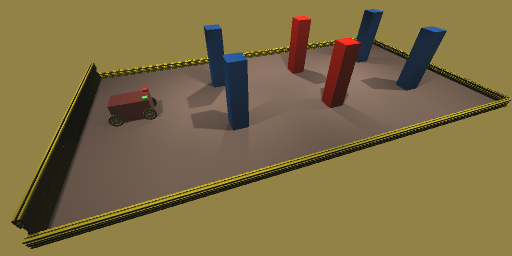
\includegraphics[width=0.3\textwidth]{Bilder/evaluation_easy.png}}\qquad
    \subfigure[Medium]{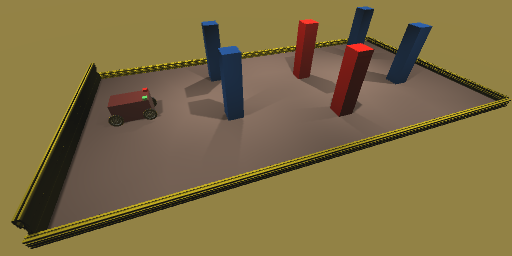
\includegraphics[width=0.3\textwidth]{Bilder/evaluation_medium.png}}\qquad
    \subfigure[Hard]{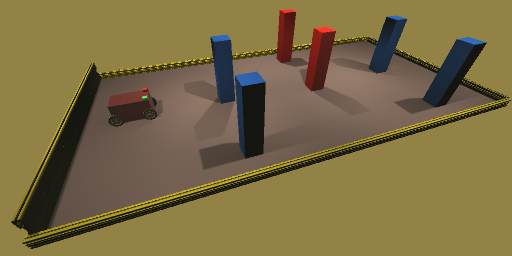
\includegraphics[width=0.3\textwidth]{Bilder/evaluation_hard.png}}\qquad
    \caption{Evaluation Tracks of different difficulties}
    \label{fig:3tracks}
\end{figure}

\subsection{Research Question 2 - Is it possible to use an end-to-end trained CNN to make the agent robust to changing light conditions?}

The evaluation parcours will be used with varying light settings to evaluate the agent's robustness towards changing light conditions. The agent's performance will be measured using the success rate, if the agent performs similarly across all light settings, the agent can be considered robust to changing light conditions.

\begin{figure}
    \centering
    \subfigure[Standard Lighting Agent POV]{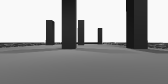
\includegraphics[width=0.3\textwidth]{Bilder/light_setting_pov_standard.png}}\qquad
    \subfigure[Standard Lighting Arena]{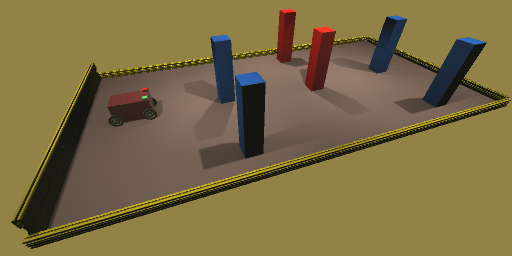
\includegraphics[width=0.4\textwidth]{Bilder/light_setting_arena_standard.png}}
    \subfigure[Reduced Lighting Agent POV]{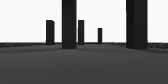
\includegraphics[width=0.3\textwidth]{Bilder/light_setting_pov_reduced_lighting.png}}\qquad
    \subfigure[Reduced Lighting Arena]{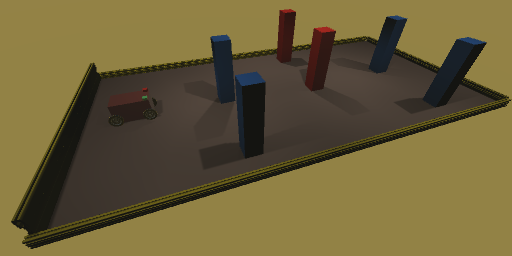
\includegraphics[width=0.4\textwidth]{Bilder/light_setting_arena_reduced_lighting.png}}
    \subfigure[Increased Lighting Agent POV]{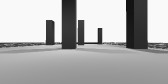
\includegraphics[width=0.3\textwidth]{Bilder/light_setting_pov_increased_lighting.png}}\qquad
    \subfigure[Increased Lighting Arena]{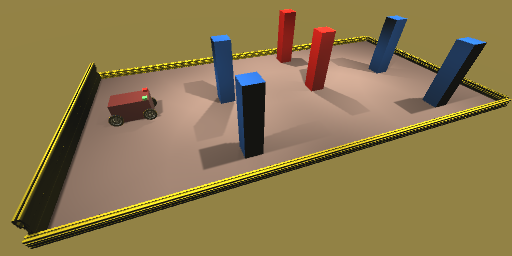
\includegraphics[width=0.4\textwidth]{Bilder/light_setting_arena_increased_lighting.png}}

    \caption{Agent Camera POV and Arena Screenshots of the different light settings} 
    \label{fig:light_settings}
\end{figure}

\subsection{Research Question 3 - Is it possible to use a neural network that can be transfered to a physical robot?}

To answer question 3, the developed agent will be evaluated on the JetBot's processing unit. There will be no physical experiments with the JetBot due to time constraints. Instead a replay of an evaluation parcour is generated in Python. The replay is then processed on the JetBot to measure its processing capabilities. The replay will consist of input-output pairs and metadata, such as processing times. If the JetBot is able to reproduce the behaviour from the replay at sufficient speed, the agent can be considered transferable to the JetBot.

% kann ich die Experimente mit varying motor power weglassen?
% die Experimente stehen nicht so stark im Zusammenhang mit den beiden Research goals
% ja
\chapter{Motivation}
\label{cha:Motivation}

The increasing utilization of artificial intelligence in academia and industry have lead to massive efficiency improvements for all kinds of tasks. The development of autonomous vehicles promises to greatly reduce the number of traffic accidents and transportation cost \autocite{mckinsey}. As a result, researchers and private enterprises from all over the globe are making progress towards fully autonomous driving agents and integrating them in commercial vehicles, many companies started to integrate adaptive cruise control and lane centering assistance \autocite{carreviews}. Due to the recent developments in artificial intelligence and the very high complexity of the task of autonomous driving, artificial intelligence often plays a big role in these systems \autocite{drl_for_ad}.


Predictions for the future of autonomous driving have been very optimistic and although huge progress has been made, the task of fully autonomous driving is still far from being solved \autocite{state_of_autonomous_driving2023}. This thesis aims at contributing to the research in this field by applying reinforcement learning to autonomous driving agents in a simulated environment. This work builds upon the work of \autocite{maximilian} and will use the same task and evaluation metrics. This thesis focusses on improving the agent's resiliency to changing light conditions by training a convolutional neural network end-to-end using reinforcement learning.
\chapter{Research Goals}
\label{cha:Research Goals}

The goal of this thesis is to contribute in the domain of autonomous driving by investigating the use of reinforcement learning to train an autonomous driving agent that is resilient to changes in light conditions. The agent is evaluated on  simulated parcours that consist of a series of goals indicated by two blocks, a parcour is successfully completed if the agents drives through all goals without collisions.
This thesis builds upon previous work at the ScaDS.AI \autocite{maximilian} and uses the same parcour and task specifications. The agent from previous work was not able to reliably complete parcours under changing light conditions, motivating the research goals of this thesis.


The self-driving agent is trained using reinforcement learning in a simulated environment, the training process will include changing light conditions and possibly data augmentation to help the agent generalize.
Parcours of different difficulties and lighting settings are used to evaluate the agent's reliability and generalisation capabilities. The most important evaluation metric is the success rate. A parcour is considered a success when the autonomous driving agent passes all goals without any collisions.


\begin{figure}
    \centering
    \subfigure{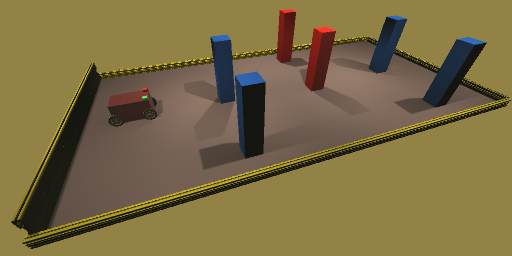
\includegraphics[width=0.4\textwidth]{Bilder/evaluation_hard.png}}\qquad
    \subfigure{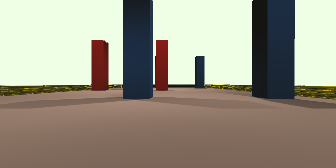
\includegraphics[width=0.4\textwidth]{Bilder/agent_image_from_unity.png}}\\
    \caption{Example image of a parcour and the agent's camera}
\end{figure}


\section{Question 1 - Is it possible to train an autonomous driving agent consisting of a convolutional neural network with end-to-end reinforcement learning to reliably solve the parcours of all difficulty levels?}

The previous work \autocite{maximilian} showed that it is possible to train an agent using reinforcement learning to solve the evaluation parcours, however the trained agents were not successful in reliably traversing the parcours of higher difficulty levels. Furthermore this work will implement the agent in a fundamentally different way, the agents developed in previous work utilized an extensive preprocessing pipeline to extract the relevant information from the camera images whereas the agents in this thesis will use a convolutional neural network to learn and extract the relevant information themselves.

Due to these differences in implementation and as a prerequisite for question 2 and 3, it is first important to investigate if it is possible to train an agent to reliably solve the parcours of all difficulty levels. This raises question 1:
Is it possible to train an autonomous driving agent consisting of a convolutional neural network with end-to-end reinforcement learning to reliably solve the parcours of all difficulty levels?

The question will be answered by training agents that have been developed based on related work and analyzing their performance on the evaluation parcours. The evaluation parcours consist of different difficulty levels, the agent's success rate will be primarily used to answer the question.


\section{Question 2 - Is it possible to use an end-to-end trained CNN to make the agent robust to changing light conditions?}

While question 1 simply investigates if it is possible to train an agent to reliably solve the parcours of all difficulty levels, question 2 investigates if it is possible to train an agent that is robust to changing light conditions in addition to being capable of solving parcours of all difficulty levels. The performance of agents from previous work \autocite{maximilian} declined massively under changing light conditions. This raises question 2 - Is it possible to use an end-to-end trained CNN to make the agent robust to changing light conditions?

The question will be answered by training agents that have been specifically designed to be robust to changing light conditions, the agents will be trained using reinforcement learning in a simulated environment with changing light conditions and possibly further data augmentation to help the agent generalize and learn. The agents will be evaluated on the evaluation parcours used in question 1 with changing light conditions. Similarly the success rate will be primarily used to evaluate and compare the agent's performance. The difference in performance for different light conditions will be used to answer the question, if the performance is similar for all light conditions the agent is considered robust to changing light conditions.

\section{Question 3 - Is it possible to use a neural network that can be transfered to a physical robot?}

One goal of the ongoing research at the ScaDS.AI is to build real life robots for demonstration and research purposes \autocite{merlin_flach}, the robots are based on the NVIDIA JetBot platform. The robots are equiped with a camera, wheels and a small computer. A future goal is to transfer a trained agent onto these robots, however the limited processing power of these robots might not be sufficient for more complex agents that utilize neural networks. This raises question 3 - Is it possible to use a neural network that can be transfered to a physical robot?


The question will be answered by investigating the processing power required to run the preprocessing steps and neural networks used in the agents that are developed in this thesis. This will be evaluated empirically by creating replays of the agents in simulations and running these replays on the physical robots. If the robots are able to reproduce the behaviour from the replays, the agents can be considered transferable to the robots.



\chapter{preprocessing Steps}
\label{cha:preprocessing Steps}

% image_printer.py erstellt die Bilder für die einzelnen Schritte/Grafiken



\newcommand{\unityImg}[1]{\makecell{\includegraphics[width=.2\linewidth]{Bilder/preprocessingSteps/fixedSpawnPoint_hardBlueFirstLeft_#1_image_from_unity.png}}}
\newcommand{\downsampledImg}[1]{\includegraphics[width=.2\linewidth]{Bilder/preprocessingSteps/fixedSpawnPoint_hardBlueFirstLeft_#1_downsampled.png}}
\newcommand{\greyscaleImg}[1]{\includegraphics[width=.2\linewidth]{Bilder/preprocessingSteps/fixedSpawnPoint_hardBlueFirstLeft_#1_greyscale.png}}
\newcommand{\equalizedImg}[1]{\includegraphics[width=.2\linewidth]{Bilder/preprocessingSteps/fixedSpawnPoint_hardBlueFirstLeft_#1_equalized.png}}
\newcommand{\finalImg}[1]{\makecell{\includegraphics[width=.2\linewidth]{Bilder/preprocessingSteps/fixedSpawnPoint_hardBlueFirstLeft_#1.png}}}


\begin{table}

    \caption{preprocessing steps applied to images from the agent camera at the different light settings. The steps are applied from top to bottom.}
    \begin{center}
        \begin{tabular}{|| c || c | c | c ||}
            \hline
            light Setting     & Bright                             & Standard                             & Dark                             \\ [0.5ex]
            \hline\hline
            Image from Unity  & \makecell{\unityImg{bright}}       & \makecell{\unityImg{standard}}       & \makecell{\unityImg{dark}}       \\
            \hline
            Downsampled       & \makecell{\downsampledImg{bright}} & \makecell{\downsampledImg{standard}} & \makecell{\downsampledImg{dark}} \\
            \hline
            Greyscale         & \makecell{\greyscaleImg{bright}}   & \makecell{\greyscaleImg{standard}}   & \makecell{\greyscaleImg{dark}}   \\
            \hline
            Equalized         & \makecell{\equalizedImg{bright}}   & \makecell{\equalizedImg{standard}}   & \makecell{\equalizedImg{dark}}   \\
            \hline
            Final Input Image & \makecell{\finalImg{bright}}       & \makecell{\finalImg{standard}}       & \makecell{\finalImg{dark}}       \\
            \hline
        \end{tabular}
    \end{center}
    \label{table:preprocessing_steps}
\end{table}


see \ref{table:preprocessing_steps} for a list of all preprocessing steps being applied to the images.






\printbibliography

% \setcounter{page}{122}
% \pagenumbering{gobble}
% %\pagenumbering{gobble}
\addchap{Erklärung}
Ich versichere, dass ich die vorliegende Arbeit mit dem Thema:

\begin{center}
\textit{\glqq\titel\grqq}\\[1em]
\end{center}
			
selbständig und nur unter Verwendung der angegebenen Quellen und Hilfsmittel angefertigt habe, insbesondere sind wörtliche oder sinngemäße Zitate als solche gekennzeichnet. Mir ist bekannt, dass Zuwiderhandlung auch nachträglich zur Aberkennung des Abschlusses führen kann. Ich versichere, dass das elektronische Exemplar mit den gedruckten Exemplaren übereinstimmt.
\par
\ort, den \eingereicht


\rule[-0.2cm]{5cm}{0.5pt}

\textsc{\autor} 
	% Selbständigkeitserklärung 

% Anhang -------------------------------------------------------------------
%		Die Inhalte des Anhangs werden analog zu den Kapiteln inkludiert.
%		Dies geschieht in der Datei Anhang.tex
% --------------------------------------------------------------------------
\appendix
\clearpage
\renewcommand*{\thesection}{\Alph{section}}
\pagenumbering{Roman}
%\include{Inhalt/Anhang}



% Index --------------------------------------------------------------------
%		Zum Erstellen eines Index, die folgende Zeile auskommentieren.
% --------------------------------------------------------------------------
%\printindex		% Index hier einfügen
%\ofoot{}
%\include{Inhalt/Thesen}	% Thesen 

\end{document}
